\textbf{Example 1}

\texttt{take\_photos(5, 7, 2, [0, 4, 4, 4, 4], [3, 4, 6, 5, 6])}

In this example we have a $7 \times 7$ grid with $5$ points of interest. 
The points of interest are located in four different cells:
$(0, 3)$, $(4, 4)$, $(4, 5)$ and $(4, 6)$. You may take at most
$2$ high-resolution photos.

One way to capture all five points of interest is to make two photos: 
a photo of the $6 \times 6$ square containing the cells $(0, 0)$ 
and $(5, 5)$, and a photo of the $3 \times 3$ square containing the
cells $(4, 4)$ and $(6, 6)$. If the satellite takes these two photos, 
it will transmit the data about $41$ cells. This amount is not optimal.

The optimal solution uses one photo to capture the $4 \times 4$ square
 containing cells $(0, 0)$ and $(3, 3)$ and another photo to capture
 the $3 \times 3$ square containing cells $(4, 4)$ and $(6, 6)$.
 This results in only $25$ photographed cells, which is optimal, so 
 `take\_photos` should return $25$.

Note that it is sufficient to photograph the cell $(4, 6)$ once, even
though it contains two points of interest.

This example is shown in the figures below. The leftmost figure shows 
the grid that corresponds to this example. The middle figure shows the
suboptimal solution in which $41$ cells were photographed. The rightmost
figure shows the optimal solution.

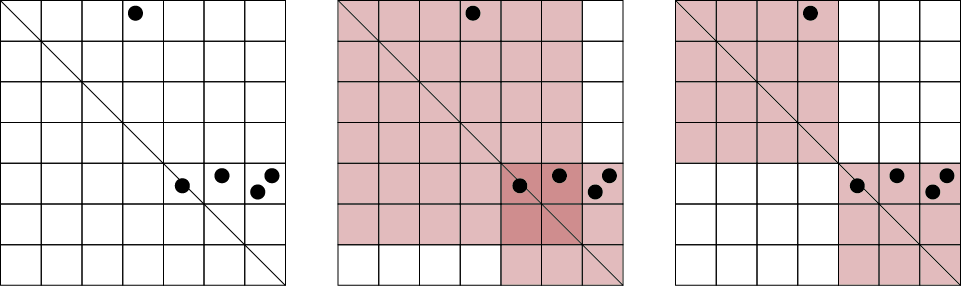
\includegraphics[scale=1.5]{example1.png}

\textbf{Example 2}

\texttt{take\_photos(2, 6, 2, [1, 4], [4, 1])}

Here we have $2$ points of interest located symmetrically: in the cells
$(1, 4)$ and $(4, 1)$. Any valid photo that contains one of them contains
the other one as well. Therefore, it is sufficient to use a single photo. 

The figures below show this example and its optimal solution.
In this solution the satellite captures a single photo of $16$ cells.

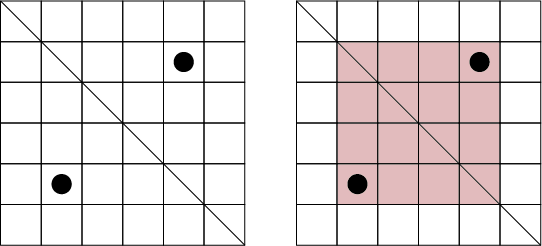
\includegraphics[scale=1.5]{example2.png}

